
\section{Friction and Applying the Laws of Motion\footnote{
1990-93 Dept. of Physics and Astronomy, Dickinson College. Supported by FIPSE
(U.S. Dept. of Ed.) and NSF. Portions of this material may have been modified
locally and may not have been classroom tested at Dickinson College.
}}

\makelabheader %(Space for student name, etc., defined in master.tex or labmanual_formatting_commands.tex)

\textbf{Objectives }

\begin{itemize}
\item To explore the characteristics of friction. 
\item To learn to use free-body diagrams to make predictions about the behavior of
systems which are acted on by multiple forces in two and three dimensions.
\end{itemize}
\textbf{Predicting and Measuring Friction Factors }

If Newton's laws are to be used to describe the sliding of a block in contact
with a flat surface, we must postulate the existence of a 
%passive 
frictional
force that crops up to oppose the applied force. There are two kinds of frictional
forces: static friction and kinetic or sliding friction, which is the friction
between surfaces in relative motion. We will concentrate on the study of kinetic
friction for a sliding block.

\textbf{Apparatus }

\begin{itemize}
\item Wooden block with hook 
\item 5.0 newton spring scale 
\item Variety of masses 
\item CS2000 compact scale
\end{itemize}
\textbf{Activity 1: Prediction of Friction Factors }

(a) List several parameters that might influence the magnitude of the kinetic
frictional force.
\vspace{20mm}

(b) Describe how you might do an experiment to determine the effect of mass
on the magnitude of the frictional force.
\vspace{20mm}

\textbf{Measuring the Effect of Mass on Kinetic Friction }

Let's determine how mass actually influences the frictional force. Perform the
experiment that you designed in the previous activity to determine how the frictional
force varies with mass. 

\newpage

\textbf{Activity 2: Friction Data and Analysis }

(a) Create a data table for the frictional force as a function of mass in the
space below. You should make at least 5-7 measurements. 
\vspace{45mm}

(b) Graph the frictional force (vertical axis) versus the mass (horizontal 
axis) and find the best fit to the data, using \textit{Excel} with a linear function. 
Print the graph and include a copy with this unit. Write the equation (with 
appropriate units) that describes the data in the space below. 
\vspace{15mm}

(c) Look up kinetic friction in your text. Read about the coefficient
of sliding friction, \( \mu _{k} \), and figure out how to determine 
\( \mu _{k} \) from the slope of your graph. Use the LINEST function in \textit{Excel} (see \textbf{Appendix \ref{excel}: Excel}) to determine the slope and its uncertainty.  Calculate \( \mu _{k} \) and its uncertainty for the block sliding on
the table. How does your range of values compare with the appropriate value in 
the table in your text? Do they agree?
\vspace{30mm}

\textbf{Theories of Friction} 

No material is perfectly ``smooth and flat.'' Any surface when
examined under a microscope is full of irregularities. It is usually assumed
that sliding friction forces result from the rubbing of rough surfaces, i.e.,
from the interlocking of surface bumps during the sliding process. How reasonable
is this explanation for sliding friction?

\textbf{Activity 3: What Surfaces Have High Friction?} 

(a) Which kinds of surfaces do you think will have the most friction rough ones
or smooth ones? Why?
\vspace{20mm}

(b) Examine the table of coefficients of friction in a text. Do the values listed
in this table support your predictions? Are you surprised? 
\vspace{20mm}

The fact that smooth surfaces sometimes have more sliding friction associated
with them than rough surfaces has led to the modern view that other factors
such as adhesion (i.e., the attraction between molecules on sliding surfaces)
also play a major role in friction. Predicting the coefficient of sliding friction
for different types of surfaces is not always possible and there is much yet
to be learned about the nature of the forces that govern sliding friction. Most
authors of introductory physics texts still tend, incorrectly, to equate smooth
surfaces with ``frictionless ones'' and to claim that the rubbing
of rough surfaces is the cause of friction.

\textbf{Free-Body Diagrams: Putting It All Together} 

You have made a series of observations which hopefully led you to reconstruct
Newton's three laws of motion and some of its ramifications for yourself. In
summary the laws are:

\textbf{Newton's First Law:} If the net force acting on an object is zero its
acceleration is zero. {[}If \( \sum  {\bf F} = 0\) then ${\bf a} = 0$
so that ${\bf v} =$ constant or zero.{]}

\textbf{Newton's Second Law:} If the net force on an object is NOT zero, then it will be accelerated according to \( \sum {\bf F} = m{\bf a}\).

\textbf{Newton's Third Law:} Any two objects that interact exert forces on each
other which are equal in magnitude and opposite in direction. {[}\textbf{F}\( _{12} \)
= -\textbf{F}\( _{21} \){]}

These three laws are incredibly powerful because an understanding of them allows
you to either: (1) use a complete knowledge of forces on a system of objects
to predict motions in the system or (2) identify the forces on a system of objects
based on observations of its motions. 

%%TB: Got rid of this, because it's wrong!  
%% Centripetal force doesn't fit into the (in my opinion nebulous anyway)
%% ``active/passive'' categorization.


%In fact, you have already used a belief
%in Newton's laws to identify several active and passive ``invisible''
%forces. The forces identified so far are shown in the table below.
%
%\vspace{0.3cm}
%{\centering \begin{tabular}{|c|c|}
%\hline 
%Active Forces&
%Passive Forces\\
%\hline 
%\hline 
%External Forces (pushes or pulls) \textbf{F}\( _{ext} \)&
%Tension Force T\\
%\hline 
%Gravitational Force \textbf{W} = m\textbf{g}&
%Normal Force \textbf{N}\\
%\hline 
%Centripetal Force \textbf{F}\( _{c} \) = m\textbf{a}\( _{c} \) = m(v\( ^{2} \)/r\( ^{2} \))(-\textbf{r})&
%Static Friction Force f = \( \mu _{s} \)N\\
%\hline 
%&
%Kinetic Friction Force f = \( \mu _{k} \)N\\
%\hline 
%\end{tabular}\par}
%\vspace{0.3cm}
%
%{\bf TO HERE}


\textbf{Using Free-Body Diagrams to Predict Motions and Calculate Forces }

The key to the effective application of Newton's laws is to identify and diagram
all the forces acting on each object in a system of interest. The next step
is to define a coordinate system and break the forces down into components to
take advantage of the fact that if \( \sum{\bf F}  = m{\bf a}\) then
\( \sum F_{x} = ma_{x} \) and \( \sum F_{y} =
ma_{y} \).

A free-body diagram consists of a set of arrows representing all the forces
on an object, but NOT the forces that the object exerts on other objects. To
create a free-body diagram you should do as follows: 

\begin{enumerate}
\item Draw arrows to represent all force acting on the object or objects in the system
of interest. 
\item Place the tail of each arrow at the point where the force acts on the object. 
\item Each arrow should point in the direction of the force it represents. 
\item The relative lengths of the arrows should, if possible, be made to correspond
to the magnitudes of the forces. 
\item A set of coordinate axis should be chosen and indicated and all of the arrows
should be labeled using standard notation to indicate the type of force involved.
\end{enumerate}
\textbf{Important Note:} The idea of using a single force vector to summarize
external forces that act in the same direction is a useful simplification which
is not real. For example, when a block rests on a table, we will say that the
table exerts a normal force on the block. It is conventional to draw a single
upward arrow at the point where the middle of the bottom surface of the block
touches the table. This arrow actually represents the sum of all the smaller
forces at each point where the block touches the table. This is shown in the
diagram below:

%\vspace{0.3cm}
{\par\centering 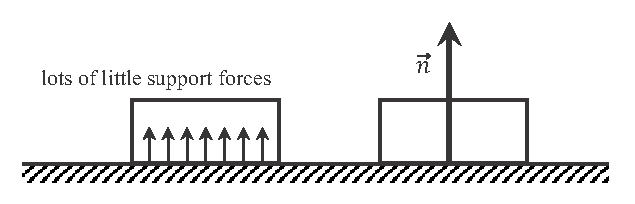
\includegraphics{friction/normal_forces.eps} \par}
\vspace{0.3cm}

\pagebreak[2]
\textbf{An Example of a Free-Body Diagram} 

Consider a block of mass $m$ sliding on a rough inclined plane as shown in the
diagram below. It has three forces on it: (1) a gravitational force, (2) a normal
force perpendicular to the surface of the plane, and (3) the friction force
opposing its motion down the plane.

Since the block is sliding it could either be moving at a constant velocity
or with a constant acceleration. Thus, it is possible that the vector sum of
forces on it is not equal to zero in some cases. For example, if there is accelerated
motion, then: \( \sum {\bf F} = {\bf N} + {\bf W} + {\bf f}
= m{\bf a}\)

%\vspace{0.3cm}
{\par\centering 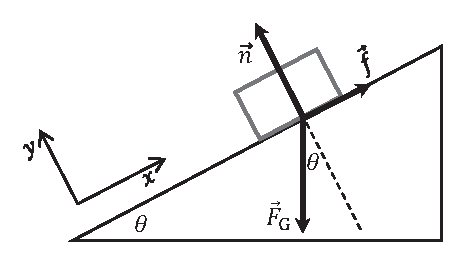
\includegraphics{friction/force_diagram.eps} \par}
%\vspace{0.3cm}

\bigskip
\textbf{Activity 4: Some Free-Body Diagrams} 

Based on the example above, try your hand at drawing the free-body diagrams for the
situations described below. In each case, write the equation for the vector
sum of forces. As always, be sure to put arrows over symbols representing vector
quantities.

(a) A block slides freely down a smooth inclined plane.

\vspace{0.3cm}
{\par\centering 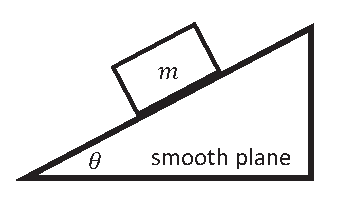
\includegraphics{friction/smooth_plane.eps} \par}
%\vspace{0.3cm}

(b) A block is on a rough plane but is not moving due to static friction.

\vspace{0.3cm}
{\par\centering 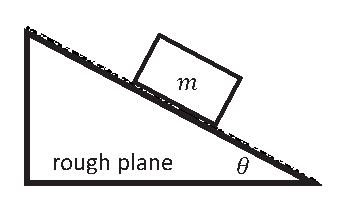
\includegraphics{friction/rough_plane.eps} \par}
%\vspace{0.3cm}

(c) A block is on a rough plane but the coefficient of friction between the
block and the plane is small. The block is sliding down the plane at a constant
velocity so that kinetic friction is acting.

\vspace{0.3cm}
{\par\centering 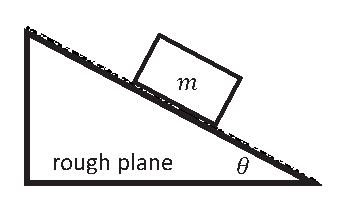
\includegraphics{friction/rough_plane.eps} \par}
%\vspace{0.3cm}

\pagebreak[2]
(d) The block is on a frictionless plane but is attached to a hanging mass of
$2m$ by one of our famous ``massless'' strings over a pulley.
Construct two free-body diagrams, one showing the forces on the mass $m$, and one showing the forces
on the mass $2m$.

\vspace{0.3cm}
{\par\centering 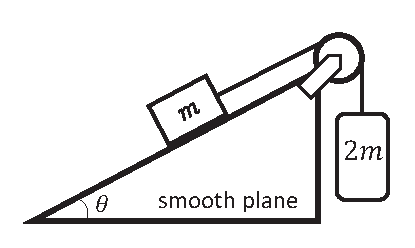
\includegraphics{friction/smooth_plane_pulley.eps} \par}
\vspace{0.3cm}

\textbf{Breaking the Forces into Components: An Example} 

Consider the case of the block sliding down a ``smooth'' plane
with a negligible amount of friction. The free-body diagram and coordinate system
chosen for analysis are shown in the figure below.

\vspace{0.3cm}
{\par\centering 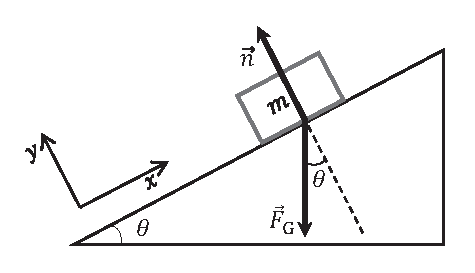
\includegraphics{friction/force_diagram2.eps} \par}
\vspace{0.3cm}

Taking components: \( W_{x}  = -W \sin  \theta  \) and \(W_{y} = -W
\cos  \theta  \).

There is no motion perpendicular to the surface so \( \sum F_y
= 0 = N + W_{y} \) so that $N = -W _{y}  = W \cos \theta$.

There is no balancing force for the x-component of W so according to Newton's
second law \( \sum F_{x}  = ma_{x} = -W \sin \theta
= - mg \sin \theta  \) and therefore \( a_{x} = - g \sin \theta  \).

\textbf{Activity 5: Solving an Inclined Plane Problem} 

(a) Consider a block sliding down a rough inclined plane at a \textbf{constant velocity}. What is the net force on it?
\vspace{20mm}

(b) Refer to the free-body diagram you created for this situation in the last
activity (part c of Activity 4). Break the forces up into components and apply Newton's first law to
find the equation for the coefficient of kinetic friction as a function of $m$,
\( \theta  \), and $g$. Remember that velocity is \textbf{constant}.

\vspace{0.3cm}
{\par\centering 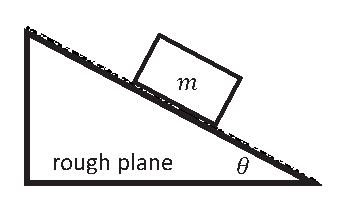
\includegraphics{friction/rough_plane.eps} \par}
\vspace{0.3cm}

